\documentclass[../main.tex]{subfiles}

\begin{document}
We are interested in automatically testing Schelling's linear segregation model. We want to answer questions such as "What is the least segregated final configuration we could reach?" or "Given an initial configuration, will this scenario \textit{converge} for any given turn function?". Furthermore, we are interested in getting the path that led to the least segregated final configuration. 

Recall, in Schelling's linear model agents are picked alternating left-most to right-most unhappy player and they will move to the closest position that makes them happy. We are going to ignore the \textit{cost} associated to moving, but we are going to keep the idea of agents moving to the closest place that make them happy since, if the moving cost were to be considered, this would generally mean least expensive move. However, when it comes to the order in which the agents get to move, we have decided to go beyond Schelling's model and look at what happens if we use different turn functions. In the previous section, we had a look at some scenarios where the different turn functions led to completely different results and in this section we are going to see if the same results are obtained by the computational model. We will ensure that all the unhappy players have equal chances to move by introducing the fairness constraint.


\begin{figure}[H]
\centering
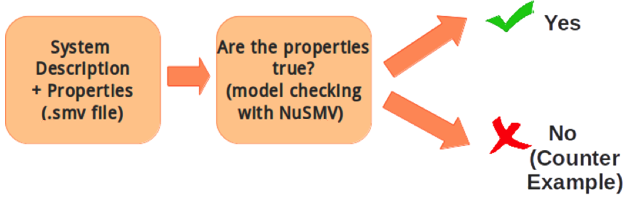
\includegraphics[scale=0.8]{NuSMV}
\caption{NuSMV Model Checker}
\end{figure}

For this project we decided to use \textit{NuSMV} model checker since it allows us to test all the possible scenarios starting from a given initial configuration, using different turn functions. The model checker creates a \textit{Binary Decision Diagram} with all the possible states following the rules of the system. As we can see in \textit{Figure 9}, the first step was to create a \verb|.smv file| with the system description and the properties written in CTL\cite[]{CTL}. Once we have the model of the system and the specifications, we can run using NuSMV, checking whether the specifications hold.

In the following sections, we are going to first explain how we modeled the linear scenario. We are going to see the SMV definitions of the line, happiness, movement turn and others. After, we are going to see at what specifications we considered and how we defined them. We needed a way to generate the \verb|.smv file| model automatically, depending only on the user inputs like number of agents, size of the local neighbourhood and the colour of the agents at each position. To do all these, we wrote a Python script at which we are going to look briefly below. 

\subsection{SMV Model}
In this section, we are going to look at the \textit{System Description} of the linear model. The system consists of a line with \verb|n| agents (the \textit{whole} world) and a local neighbourhood size \verb|s|. Our model needs to initialise the positions of the line as passed in from the user, \verb|i.e.| the user decides how many players are there and what type (colour) each player is. The model also has to define the rules that determine whether an agent is happy or not and positions he could move to. It defines which are the new potential locations for an agent, that is, which positions are the nearest and make the agent happy. For this model, we defined two modules: a \textit{main module} and a \textit{line module}. Each module is an encapsulated description that can be instantiated within the model. The module \textit{main} forms the root of the model hierarchy and the starting point for building the finite-state model. We have declared local variables within each module and we defined the value of each of these variables in each state using \verb|init| and \verb|next|. Below, we are going to analyse and give a small example for each of these two modules and then look at the fairness constraint we needed. \\


\textbf{MODULE line}

This module encodes the agents in the line. As we see below, we have a variable line which is an array with \verb|n| positions and each element of the array can be either 0 or 1; 0 for white and 1 for black. So \verb|line[3] = 0| represents that the person at position 3 is white. It also has a Boolean array called \verb|happy| representing the happiness status of each position in the line. So, for example, \verb|happy[3] = TRUE| represents that fact that the player on position 3 is happy. Furthermore, we can see that the module takes as input \verb|old_pos| (the current position of the person to move) and \verb|new_pos| (the new position of the person to move).
\begin{lstlisting}
MODULE line(old_pos,new_pos)
  VAR
    line  : array 1..n of 0..1;
    happy : array 1..n of boolean;
  ASSIGN
-- Initialise the line, i.e. the first configuration 
    init(line[1]) := 1;
    init(line[2]) := 0;
    ...
    init(line[n]) := 1;
    
-- This is how the colours change in the line when the person in
-- old_pos moves to new_pos.  
    next(line[1]) :=
      case
        new_pos = 1 : line[old_pos]; 
        new_pos > old_pos & 1 >= old_pos & 1 < new_pos : line[2];
        TRUE : line[1];
      esac;
    next(line[2]) :=
      case
        new_pos =  2 : line[old_pos];
        new_pos > old_pos &  2 >= old_pos &  2 < new_pos : line[3];
        new_pos < old_pos & 2 > new_pos & 2 <= old_pos : line[1];
        TRUE : line[2];
      esac; 
    ...
    next(line[n]) :=
      case
        new_pos = n : line[old_pos]; 
        new_pos < old_pos & n > new_pos & n <= old_pos : line[n];
        TRUE : line[n];
      esac;

-- Initialise happiness statuses for a local neighbourhood of size 1, 
-- i.e. each person cares about the colour of the person at 
-- his right and the person at his left
    init(happy[1]) :=
      case 
        line[1] = 0 & line[2]  <= 0 : TRUE;
        line[1] = 1 & line[2]  >= 1 : TRUE;
        TRUE: FALSE;
      esac;
    init(happy[2]) :=
      case 
        line[2] = 0 & line[1] + line[3] <= 1 : TRUE;
        line[2] = 1 & line[2] + line[3] >= 1 : TRUE;
        TRUE: FALSE;
      esac;
    ...
    init(happy[n]) :=
      case 
        line[n] = 0 & line[n-1] <= 0 : TRUE;
        line[n] = 1 & line[n-1] >= 1 : TRUE;
        TRUE: FALSE;
      esac;


-- This is how the hapiness statuses change in the line when the person in
-- old_pos moves to new_pos.
    next(happy[1]) :=
      case 
        next(line[1]) = 0 & next(line[2]) <= 0 : TRUE;
        next(line[1]) = 1 & next(line[2]) >= 1 : TRUE;
        TRUE: FALSE;
      esac;
    next(happy[2]) :=
      case 
        next(line[2]) = 0 & next(line[1]) + next(line[3]) <= 1 : TRUE;
        next(line[2]) = 1 & next(line[1]) + next(line[3]) >= 1 : TRUE;
        TRUE: FALSE;
      esac;
    ...
    next(happy[3]) :=
      case 
        next(line[n]) = 0 & next(line[n-1]) <= 0 : TRUE;
        next(line[n]) = 1 & next(line[n-1]) >= 1 : TRUE;
        TRUE: FALSE;
      esac;
\end{lstlisting}



\textbf{MODULE main} 

 There are three local variables: old position, new position and persons. The old and new position variable take an integer value between 1 and n, where n is the total number of agents, and the variable persons represents the people in a line. \verb|persons| is an instance of the module \verb|line|. This allows us to build a structural hierarchy. Here is a small example of the main module for just 3 agents, \verb|n = 3|, and local neighbourhood size of 1, \verb|s = 1|, that is, each agent is interested in the type of the two agents that are the closest, one on his right and one on his left. Recall, we say that an agent is happy if at least 50\% of his neighbours are like oneself.
\begin{lstlisting}
MODULE main
  VAR
    old_pos: 1..3;
    new_pos: 1..3;
    change : boolean; 
    persons: line(old_pos,new_pos);

  ASSIGN
    init(new_pos) :=
      case
        old_pos=1 & persons.happy[1] = TRUE : 1;
        old_pos=1 & persons.happy[1] = FALSE & persons.line[1] = 0 &  persons.line[2] + persons.line[3] <= 1 : {2};
        old_pos=1 & persons.happy[1] = FALSE & persons.line[1] = 1 &  persons.line[2] + persons.line[3] >= 1 : {2};
        old_pos=1 & persons.happy[1] = FALSE & persons.line[1] = 0 & persons.line[3] <= 0 : {3};
        old_pos=1 & persons.happy[1] = FALSE & persons.line[1] = 1 & persons.line[3] >= 1 : {3};
        old_pos=2 & persons.happy[2] = TRUE : 2;
        old_pos=2 & persons.happy[2] = FALSE & persons.line[2] = 0 & persons.line[1] <= 0 & persons.line[3] <= 0 : {1,3};
        old_pos=2 & persons.happy[2] = FALSE & persons.line[2] = 1 & persons.line[1] >= 1 & persons.line[3] >= 1 : {1,3};
        old_pos=2 & persons.happy[2] = FALSE & persons.line[2] = 0 & persons.line[1] <= 0 : {1};
        old_pos=2 & persons.happy[2] = FALSE & persons.line[2] = 1 & persons.line[1] >= 1 : {1};
        old_pos=2 & persons.happy[2] = FALSE & persons.line[2] = 0 & persons.line[3] <= 0 : {3};
        old_pos=2 & persons.happy[2] = FALSE & persons.line[2] = 1 &  persons.line[3] >= 1 : {3};
        old_pos=3 & persons.happy[3] = TRUE : 3;
        old_pos=3 & persons.happy[3] = FALSE & persons.line[3] = 0 & persons.line[1] + persons.line[2] <= 1 : {2};
        old_pos=3 & persons.happy[3] = FALSE & persons.line[3] = 1 & persons.line[1] + persons.line[2] >= 1 : {2};
        old_pos=3 & persons.happy[3] = FALSE & persons.line[3] = 0 & persons.line[1] <= 0 : {1};
        old_pos=3 & persons.happy[3] = FALSE & persons.line[3] = 1 & persons.line[1] >= 1 : {1};
        TRUE : old_pos;
    esac;

    next(new_pos) :=
      case
        next(old_pos)=1 & next(persons.happy[1]) = TRUE : 1;
        next(old_pos)=1 & next(persons.happy[1]) = FALSE & next(persons.line[1]) = 0 & next(persons.line[2]) + next(persons.line[3]) <= 1 : {2};
        ...
        next(old_pos)=3 & next(persons.happy[3]) = FALSE & next(persons.line[3]) = 1 & next(persons.line[1]) >= 1 : {1};
        TRUE : next(old_pos);
    esac;
      
\end{lstlisting}


The \verb|old_pos| variable is chosen arbitrary between 1 and n, where n is the total number of agents. If, at a step, the \verb|olp_pos = 3|, then this represents that is the turn of person on position 3 to move. If the agent at position 3 is happy, (\verb|i.e. persons.happy[3] = TRUE|), then the player will remain in the same position, (\verb|i.e.| we set the value of the \verb|new_pos| variable above to 3). Otherwise, if the agent is not happy, we find the nearest position that makes him happy. We do this from nearest to further. Notice, if there are two equidistant positions that would satisfy the agent then, it can choose randomly between the two positions. In the example below, if it is the turn for player 2 to move and player two is 0 (black) and both position 1 and 3 would meet his demands then it can be chosen randomly between the two positions.

\begin{lstlisting}
old_pos=2 & persons.happy[2] = FALSE & persons.line[2] = 0 & persons.line[1] <= 0 & persons.line[3] <= 0 : {1,3};
\end{lstlisting}

\textbf{Fairness constraints}

At this stage, we can see that an incorrect behaviour might occur. This would corresponds to circumstances that are not of interest, like same player getting to move over and over again. Thus, we have to assume \textit{fairness} for all the agents in the model. We were able to do so by simply adding the following constraints.

\begin{lstlisting}
  FAIRNESS old_pos = 1
  FAIRNESS old_pos = 2
  FAIRNESS old_pos = 3
  ...
  FAIRNESS old_pos = n
\end{lstlisting}

\verb|FAIRNESS old_pos = p| indicates that only paths in which \verb|old_pos = p| happens infinitely often will be traversed. This is enough to ensure that each player will get to move infinitely often. \\


\subsection{CTL Specifications}
We first had to consider what properties are we interested in checking, whether they hold or not in our model of the system. Firstly, and very important, we want to look at whether or not the system will converge in all scenarios. The system \textit{converges} if it reaches a terminal state. A terminal state is a state in which no unhappy player is able to improve. Secondly, we are interested in how segregated the final configurations are. We want final configurations that are as least segregated as possible. We are now going to look at what other variables we introduced in order to check the above statements and what specifications we have written.\\

\subsubsection{Convergence}

 To check convergence, we introduced a Boolean variable in the main module called \verb|change|. This Boolean variable is \textit{true} if at least one player has changed his position, \textit{false} otherwise. Here is how it is defined.
 
 \begin{lstlisting}
    change : boolean;
     ...
    init(change) := FALSE;
    
    next(change) := 
      case
        next(old_pos) != next(new_pos) : TRUE;
        TRUE : FALSE;
      esac; 
 \end{lstlisting}
 
 And here is the CTL specification we wrote.
 
 \begin{lstlisting}
 SPEC
  AF AG (!change);
 \end{lstlisting}
 
 Translating this specification from CTL to \textit{English}, would be the following: "For all the possible paths, there will be a point in the future where \verb|change| will always be false". In other words, in all the paths, we will reach a point where nobody will move any longer.\\
 
\subsubsection{Degree of Segregation}
 
 In order to check how segregated our model is, we introduced a new variable  \verb|segregation_table| in the \verb|MODULE line|. This variable is an array of zeros and ones. The size of the array is \verb|n-1|, where \verb|n| is the total number of agents. Here is how we defined it.
 
 \begin{lstlisting}
    separation_table : array 1..n-1 of 0..1;
    ...
    init(separation_table[1]) := 
      case 
        line[1] != line[2] : 1;
        TRUE : 0;
      esac;
    
    init(separation_table[2]) := 
      case 
        line[2] != line[3] : 1;
        TRUE : 0;
      esac;
    ...
    init(separation_table[n-1]) := 
      case 
        line[n-1] != line[n] : 1;
        TRUE : 0;
      esac;
    
    next(separation_table[1]) := 
      case 
        next(line[1]) != next(line[2]) : 1;
        TRUE : 0;
      esac;
    
    next(separation_table[2]) := 
      case 
        next(line[2]) != next(line[3]) : 1;
        TRUE : 0;
      esac;
    ...
    next(separation_table[n-1]) := 
      case 
        next(line[n-1]) != next(line[n]) : 1;
        TRUE : 0;
      esac;

 \end{lstlisting}
 
 In the \verb|separation_table| array we store ones if there is a colour change, zeros otherwise. In other words, \verb|separation_table[3] = 1| means that the person on position three has a different colour than person on position 4.
 
 Given the following configuration
 \begin{table}[H]
\begin{center}
{\begin{tabular}{| c |c| c| c| c |c| c |c|}
\hline
\z &\z &\x &\x  &\z &\x &\z & \x \\
 \hline
\end{tabular}}
\end{center}
\end{table}

The \verb|separation_table| will look like this:
 \begin{table}[H]
\begin{center}
{\begin{tabular}{| c |c| c| c| c |c| c |}
\hline
0 & 1 & 0 & 1  & 1 & 1 & 1  \\
 \hline
\end{tabular}}
\end{center}
\end{table}

This new variable allows us to write specifications to answer questions like \textit{"Is complete segregation possible?"}. We say we have a \textbf{complete segregation} when all the whites form a contiguous group and all the black form another contiguous group. Hence we can define complete segregation as the sum of all the elements of the array \verb|separation_table| being equal to 1, or 0 if everybody in the model is of the same colour. \\


\textbf{Complete Segregation:}

\verb|separation_table[1] + ... + separation_table[n-1] = 1 or 0| (It is equal to 0 in a special case where all agents are of the same type. This case is not of interest to us, but we will consider it in the specification)

 And here is how we would write the specification in CTL to check complete segregation:
 \begin{lstlisting}
SPEC
  AF AG (
  persons.separation_table[1] + ... + persons.separation_table[n-1] = 1 |
  persons.separation_table[1] + ... + persons.separation_table[n-1] = 0 );
 \end{lstlisting}

This specification checks that for all the paths, there will be complete segregation at some point. 

\begin{figure}[H]
\centering
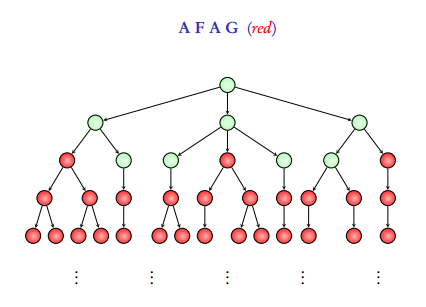
\includegraphics[scale=0.8]{afag}
\caption{For all paths, red is eventually true forever \cite[]{ctl_picture}}
\end{figure}


We also want to check what is the least segregated, final configuration  we can reach. We check the sum of the elements of the \verb|separation_table| array all the way up to n-1, that is, the largest value we can get and it is reachable when whites and blacks are alternating (\verb|i.e.| one white, one black, one white, one black,...). In other words, all the elements of the \verb|separation_table| array will equal to 1 if we have the agents in the line alternating black, white.
 \begin{lstlisting}
SPEC
  EF AG (
  persons.separation_table[1] + ... + persons.separation_table[n-1] = 1 );

SPEC  
  EF AG (
  persons.separation_table[1] + ... + persons.separation_table[n-1] = 2 );
  
  ...

SPEC  
  EF AG (
  persons.separation_table[1] + ... + persons.separation_table[n-1] = n-1 );
 \end{lstlisting}

\verb|EF AG p| means that \textit{there exists a future point from which, in all the future paths, p will hold}. 
\begin{figure}[H]
\centering
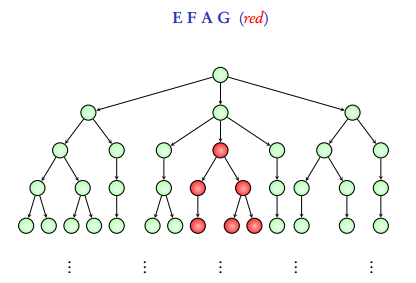
\includegraphics[scale=0.8]{efag}
\caption{There exists a path such that red is eventually true forever \cite[]{ctl_picture}}
\end{figure}

\begin{lstlisting}
SPEC  
  EF AG (
  persons.separation_table[1] + ... + persons.separation_table[n-1] = 2 );
 \end{lstlisting}
Hence, the above specification checks whether there is a final configuration with three groups, that is, something like this:
  
 \begin{table}[H]
\begin{center}
{\begin{tabular}{| c |c| c| c| c |c| c |c|c|c|c|}
\hline
\z &\z & \z & ...  &\x &\x &\x & ... &\z&\z&\z \\
 \hline
\end{tabular}}
\end{center}
\end{table} 

Once we got the highest number, the least segregated final configuration, we could use NuSMV to generate the path that led to that configuration. In other words, we can ask NuSMV to give us the best scenario where the final configuration is least segregated.


A complete \verb|.smv file| example can be found at Appendix \ref{appendix:smv}.

\subsection{Python Script}
In the sections above, we had a look at how we designed the model of the system and what does the \verb|.smv file| includes in terms of System Description and Properties. However, SMV has some limitations such as the \textit{main} module which forms the root of the model hierarchy does not take any parameters. Furthermore, SMV does not support control flow statements, such as \verb|for- | or \verb|while- | loops. Therefore, we would needed to write a new file, create a new model, for each configuration we want to represent. It was natural to use another programming language that allows control flow statements and can take user inputs and generate the \verb|.smv file|. We chose \textit{Python}\cite[]{Python}.  

We use the following user inputs:
\begin{itemize}
    \item The number of agents we have in the line
    \item The size of the local neighbourhood 
    \item The initial configuration, \verb|i.e.| the colour of the person at each position
\end{itemize}

\begin{figure}[H]
\centering
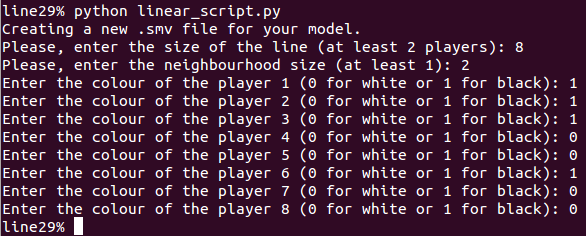
\includegraphics[scale=0.8]{python_script}
\caption{Example of user input when running the Python script}
\end{figure}

For each local variable in the model, we wrote Python functions which, based on the input values, are able to define the values of these variables in each state. 



\end{document}